\chapter{Estudo de Caso}
\label{estudo de caso}


\citeonline{wohlin2012experimentation} enuncia a necessidade que uma metodologia de estudo de caso, definida formalmente em engenharia de software, deva conter os passos da Figura \ref{fig:metodologia-estudo}.

\begin{figure}[ht!]
\centering
\includegraphics[keepaspectratio=true,scale=0.16]{figuras/metodologia-estudo-caso.eps}
\caption{Metodologia de Estudo de Caso proposta por \citeonline{wohlin2012experimentation}}
\label{fig:metodologia-estudo}
\end{figure}
\FloatBarrier

\section{Planejamento do Estudo de Caso}
\label{sec:planning-case}
Para o planejamento do estudo de caso em engenharia de software é essencial, segundo \citeonline{brereton2008using}, que se descreva o protocolo do estudo de caso. Este consiste em um relatório simplificado das principais variáveis, dados e passos, tais como o meio e modo de coleta de dados, identificação das fontes de dados e formas de análise de dados \cite{wohlin2012experimentation}. 


O protocolo de estudo de caso deste trabalho, que foi baseado em \citeonline{brereton2008using} e \citeonline{wohlin2012experimentation} foi dividido em seções, conforme se vê a seguir.


\subsection{Trabalhos Relacionados ao Estudo de Caso}

Assim como os trabalhos de \citeonline{Palza2003}, \citeonline{Ruiz2005}, \citeonline{Castellanos2005}, \citeonline{Becker2006}, \citeonline{Folleco2007}, \citeonline{Silveira2010}, buscou-se alcançar uma validação empírica da utilização ambiente de \textit{Data Warehousing} proposto no Capítulo \ref{chap:arquitetura}.


\subsection{Objetivos do Estudo de Caso}

O objetivo geral do estudo de caso foi avaliar um software durante o seu desenvolvimento no ambiente de \textit{Data Warehousing} proposto no Capítulo \ref{chap:arquitetura}. Em consonância ao objetivo geral do estudo de caso e aos objetivos específicos deste trabalho, foram definidos objetivos específicos do estudo de caso, tal como se mostra na Tabela \ref{tab:objetivos-estudo-de-caso}.

\begin{table}[H]
\begin{center}
\input{tabelas/objetivos-estudo.ltx}
\caption{Objetivos Específicos de Estudo de Caso}
\label{tab:objetivos-estudo-de-caso}
\end{center}
\end{table}
\FloatBarrier

\subsection{Seleção de Objeto do Estudo de Caso} 

Para selecionar o software que seria parte da avaliação do ambiente de \textit{Data Warehousing} que é o objeto do estudo de caso, foram considerados os critérios estabelecidos na Tabela \ref{tab:critérios-estudo-de-caso}. 


\begin{table}[H]
\begin{center}
\input{tabelas/criterios-estudo.ltx}
\caption{Critérios de Seleção de Objeto do Estudo de Caso}
\label{tab:critérios-estudo-de-caso}
\end{center}
\end{table}
\FloatBarrier

\subsection{Objeto de Estudo}

\subsubsection{Visão Geral}

O IPHAN é autarquia federal responsável pela gestão de diversos processos de preservação do patrimônio cultural, como por exemplo,ações para sua identificação, proteção, gestão e fomento. Decorrente
de suas atribuições, o órgão produz uma grande quantidade de informações fragmentadas em termos territoriais e temáticos. Nos últimos quatro anos, o IPHAN elaborou uma metodologia
para definir os processos de cadastro, inventário e gestão do patrimônio cultural material. Essa metodologia tem por objetivo geral abordar o Patrimônio Cultural de forma integrada, sistêmica
e estratégica, conforme detalhado a seguir:

\begin{itemize}
\item Integrada: cobrindo todas as categoriais do patrimônio material;
\item Sistêmica: estabelecendo moldes a serem utilizados nas diversas etapas de ações de preservação, possibilitando o "diálogo" e troca de informações entre áreas e etapas de trabalho;
\item Estratégica: considerando o mapeamento, a organização e a disponibilização de informações sobre o patrimônio como base para a construção de políticas públicas integradas - com outros parceiros - e de planos de preservação e desenvolvimento das regiões onde se inserem os bens.
\end{itemize}

Em termos específicos, a metodologia buscou, em primeiro lugar, mapear os procedimentos necessários para a execução das ações de cadastramento, proteção, normatização e fiscalização de bens culturais de natureza material, indicando adicionalmente os dados a serem coletados. Este mapeamento contou com a participação de representantes das Superintendências e Escritórios Técnicos, que, por meio de Grupos de Trabalho, analisaram, de forma crítica, as metodologias até então existentes.

A revisão dos processos levou à formulação da nova metodologia que, por sua vez, permitiu a otimização das atividades de cadastramento de sítios históricos e de bens tombados isoladamente e gerou a normalização das ações de fiscalização. O resultado desse trabalho produziu um conjunto de fichas e procedimentos específicos com demandas para cadastramento de dados textuais, geográficos e imagens.

Há um entendimento no IPHAN de que é necessária a formação de uma rede de proteção fomentada pelo SNPC que consolide o grande volume de informações atualmente produzido por suas unidades administrativas, composto de 27 Superintendências, 30 escritórios técnicos, 4 Unidades Especiais e 2 Parques Históricos Nacionais. Entretanto, na conjuntura atual, a natureza das informações, em grande maioria armazenadas em planilhas e em banco de dados isolados, dificulta o processo de consolidação das informações, fato 
que impede a construção da rede de proteção baseada nos recursos e tecnologias atualmente adotados, pois demandaria o aporte considerável de recursos financeiros e humanos sem ganhos no processo. O órgão se manteria refém da demora na produção de informações decorrente do intervalo entre ação e recepção das respostas, ou seja, entre a percepção do problema e sua solução.

Apesar do fato de os processos de cadastramento, normatização de sítios urbanos tombados e fiscalização de bens imóveis de metodologia já fazerem parte da realidade das Superintendências e Escritórios Técnicos, o processo manual de suporte e gestão dos dados torna a execução precária e morosa.

\subsubsection{O Software Analisado}

Tendo em vista a dificuldade que o processo manual acarreta, o IPHAN decidiu contratar uma empresa de software para desenvolver uma solução que pudesse automatizar o processo de trabalho decorrente da metodologia de inventário, cadastramento, normatização, fiscalização, planejamento e análise e gestão do patrimônio material. Esta solução de software foi concebida sobre a denominação de Sistema Integrado de Conhecimento e Gestão (SICG) que foi construído em Java (atende-se ao critério CEC1), durante 24 \textit{releases} mensais (atende-se ao critério CEC2), utilizando \textit{frameworks} como VRaptor, Hibernate formado por 7 módulos:

\begin{itemize}
\item Módulo de Conhecimento;
\item Módulo de Análise e Gestão;
\item Módulo de Cadastro;
\item Módulo de Administração de Usuários;
\item Módulo de Fiscalização;
\item Módulo de Cadastro Auxiliares;
\item Módulo de Relatórios Adicionais.
\end{itemize}


\subsection{Dados, Fonte dos Dados e Forma de Análise dos Dados}

Após a identificação dos objetivos do estudo de caso, foram identificados os principais dados qualitativos e quantitativos na Tabela \ref{tab:dados-estudos}. Estes são as respostas que espera obter com o monitoramento e avaliação de métricas de código-fonte e cenários de limpeza de código-fonte em um ambiente de \textit{Data Warehousing}.


\begin{table}[H]
\begin{center}
\input{tabelas/dados-estudo.ltx}
\caption{Dados do Estudo de Caso}
\label{tab:dados-estudos}
\end{center}
\end{table}
\FloatBarrier

\subsection{Ameaças à Validade do Estudo de Caso}
\label{sec:validade-estudo}

\citeonline{yin2011applications} destaca que há quatro ameaças a realização de estudos de caso: Validade de Construção, Validade Interna, Validade Externa e de Confiabilidade.

A validade de construção está presente na fase de coleta de dados onde deve ser evidenciado as múltiplas fontes de evidência e a coleta de um conjunto de métricas para que se possa saber exatamente o que medir e quais dados são relevantes para o estudo, de forma a responder as questões de pesquisa \cite{yin2011applications}. Neste trabalho, buscou-se garantir a validade de construção ao se definir objetivos com evidências diferentes. Estas por sua vez estão diretamente relacionadas com os objetivos do estudo de caso e os objetivos do trabalho conforme mostrado na Tabela \ref{tab:objetivos-estudo-de-caso}.

A validade interna é garantida quando as conclusões apresentadas pelo estudo de caso correspondem a alguma realidade conhecida pelos próprios envolvidos no projeto \cite{yin2011applications}. Neste trabalho, procurou-se atender a validade interna com a triangulação de vários indicadores de qualidade de código-fonte, isto é, a correlação entre diversos métodos de análise que podem levar conclusões equivalentes. 

Quanto a validade externa destaca-se que a utilização de um estudo de caso não é suficiente para generalizar os resultados dele obtidos, sendo necessário a utilização de estudo em múltiplos casos, a fim de comprovar a genericidade dos resultados \cite{yin2011applications}. Embora, como citado anteriormente, alguns trabalhos já trabalharam com a utilização de métricas e ambientes de \textit{Data Warehousing}, não há como correlacionar os resultados obtidos devido a grande diferenças de contexto e aplicação do ambiente, logo a validade externa não é garantida neste trabalho.

Com relação a confiabilidade, \citeonline{yin2011applications} enuncia que para se garantí-la em um estudo de caso, é necessário que este tenha repetibilidade caso seja usada a mesma fonte dos dados. Neste trabalho, com a documentação da implementação do ambiente de \textit{Data Warehousing}, presente no Capítulo \ref{chap:arquitetura}, conjuntamente com o protocolo de estudo de caso, apresentado a partir da Seção \ref{sec:planning-case}, garante-se a repetibilidade do estudo de caso e por conseguinte a confiabilidade.

\section{Execução do Estudo de Caso e Análise dos Dados}
\label{sec:execution-case-study}

Para cada uma das \textit{releases} do SICG, coletou-se o código-fonte, conforme a disponibidilidade, em um servidor FTP cedido pelo IPHAN. Em alguns casos, o próprio IPHAN não possuía o código-fonte de uma determinada \textit{release} tal como se mostra na Figura \ref{fig:repositorio-IPHAN}.

\begin{figure}[ht!]
\centering
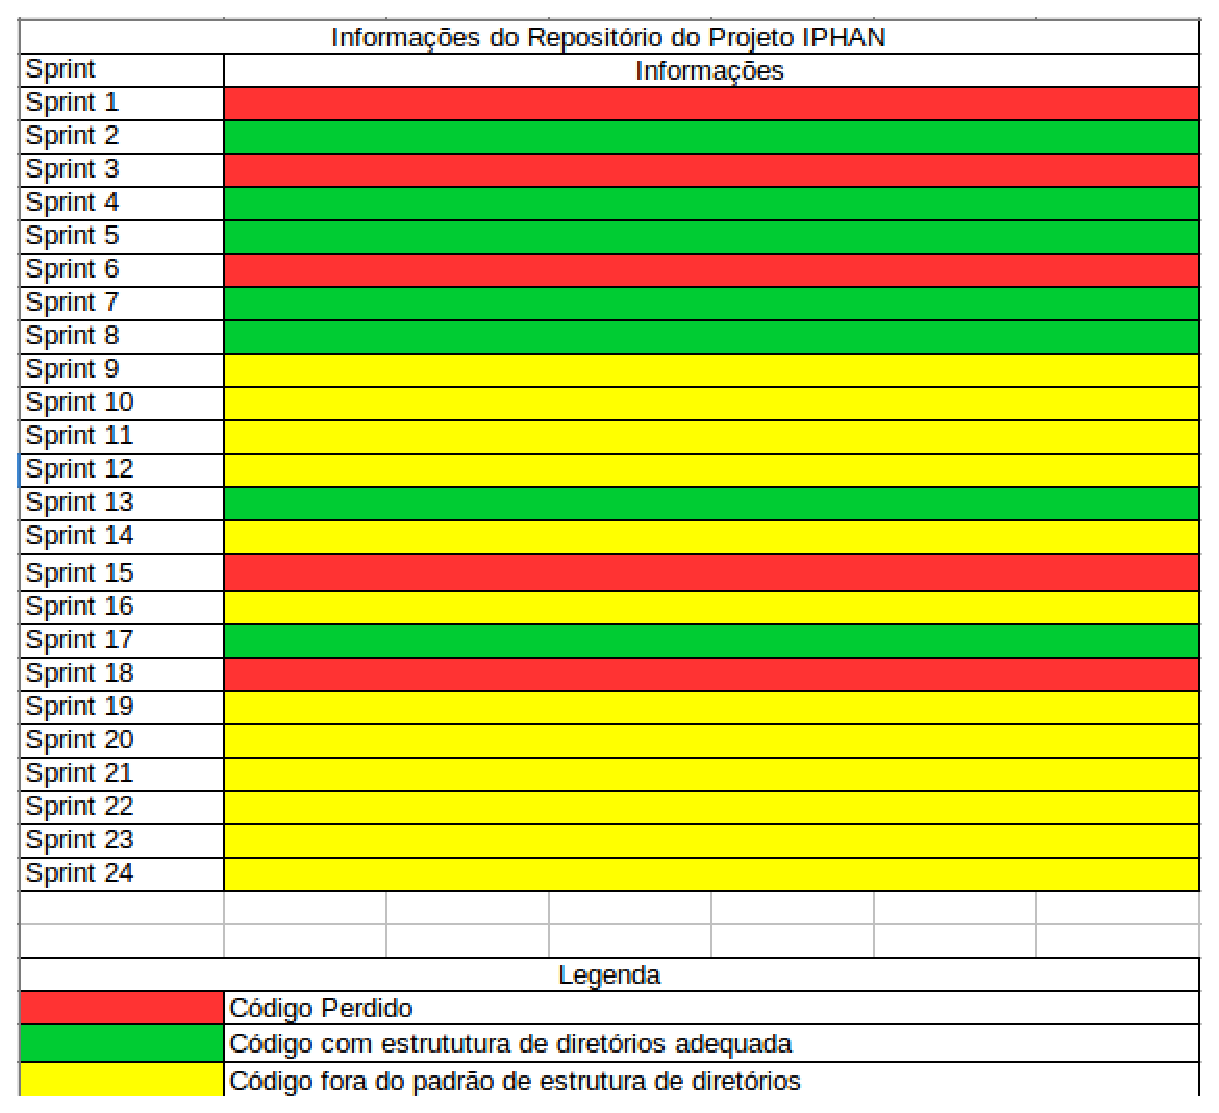
\includegraphics[keepaspectratio=true,scale=0.5]{figuras/repositorio-iphan.eps}
\caption{Informações do Repositório de Código-Fonte}
\label{fig:repositorio-IPHAN}
\end{figure}
\FloatBarrier


Após o código-fonte de cada versão ser coletado, foi feita uma análise da estrutura de diretórios, a fim de obter uma padronização na análise das métricas de código-fonte. Em casos que foram marcados com amarelos conforme a Figura \ref{fig:repositorio-IPHAN}, a estrutura de diretórios não estava condizente com a adotada pelo projeto, sendo necessário a correção para que as análises de código-fonte pudessem ser executadas corretamente. Posteriormente, os dados obtidos da análise estática do código-fonte foram carregados no ambiente de \textit{Data Warehousing} proposto no Capítulo \ref{chap:arquitetura}. Dessa forma, foi possível obter para cada \textit{release} que estava com código-fonte presente: Valor Percentil para cada uma das Métricas de Código-Fonte, Quantidade de Cenários de Limpeza presentes em uma determinada Classe do Projeto e o cálculo da Taxa de Aproveitamento de Oportunidade de Melhoria de Código-Fonte. 


\subsection{Análise dos Valores Percentis para Métricas de Código-Fonte do SICG}

Após extrair as métricas do código-fonte, obteve-se valores percentis para as configurações~"OpenJDK8 Metrics"~e~"Tomcat Metrics"~, que foram definidas na Tabela \ref{tab:good-metrics}, conforme mostra as Figuras \ref{fig:total-openJDK8} e \ref{fig:total-tomcat}   
respectivamente.

\begin{sidewaysfigure}[ht!]
\centering
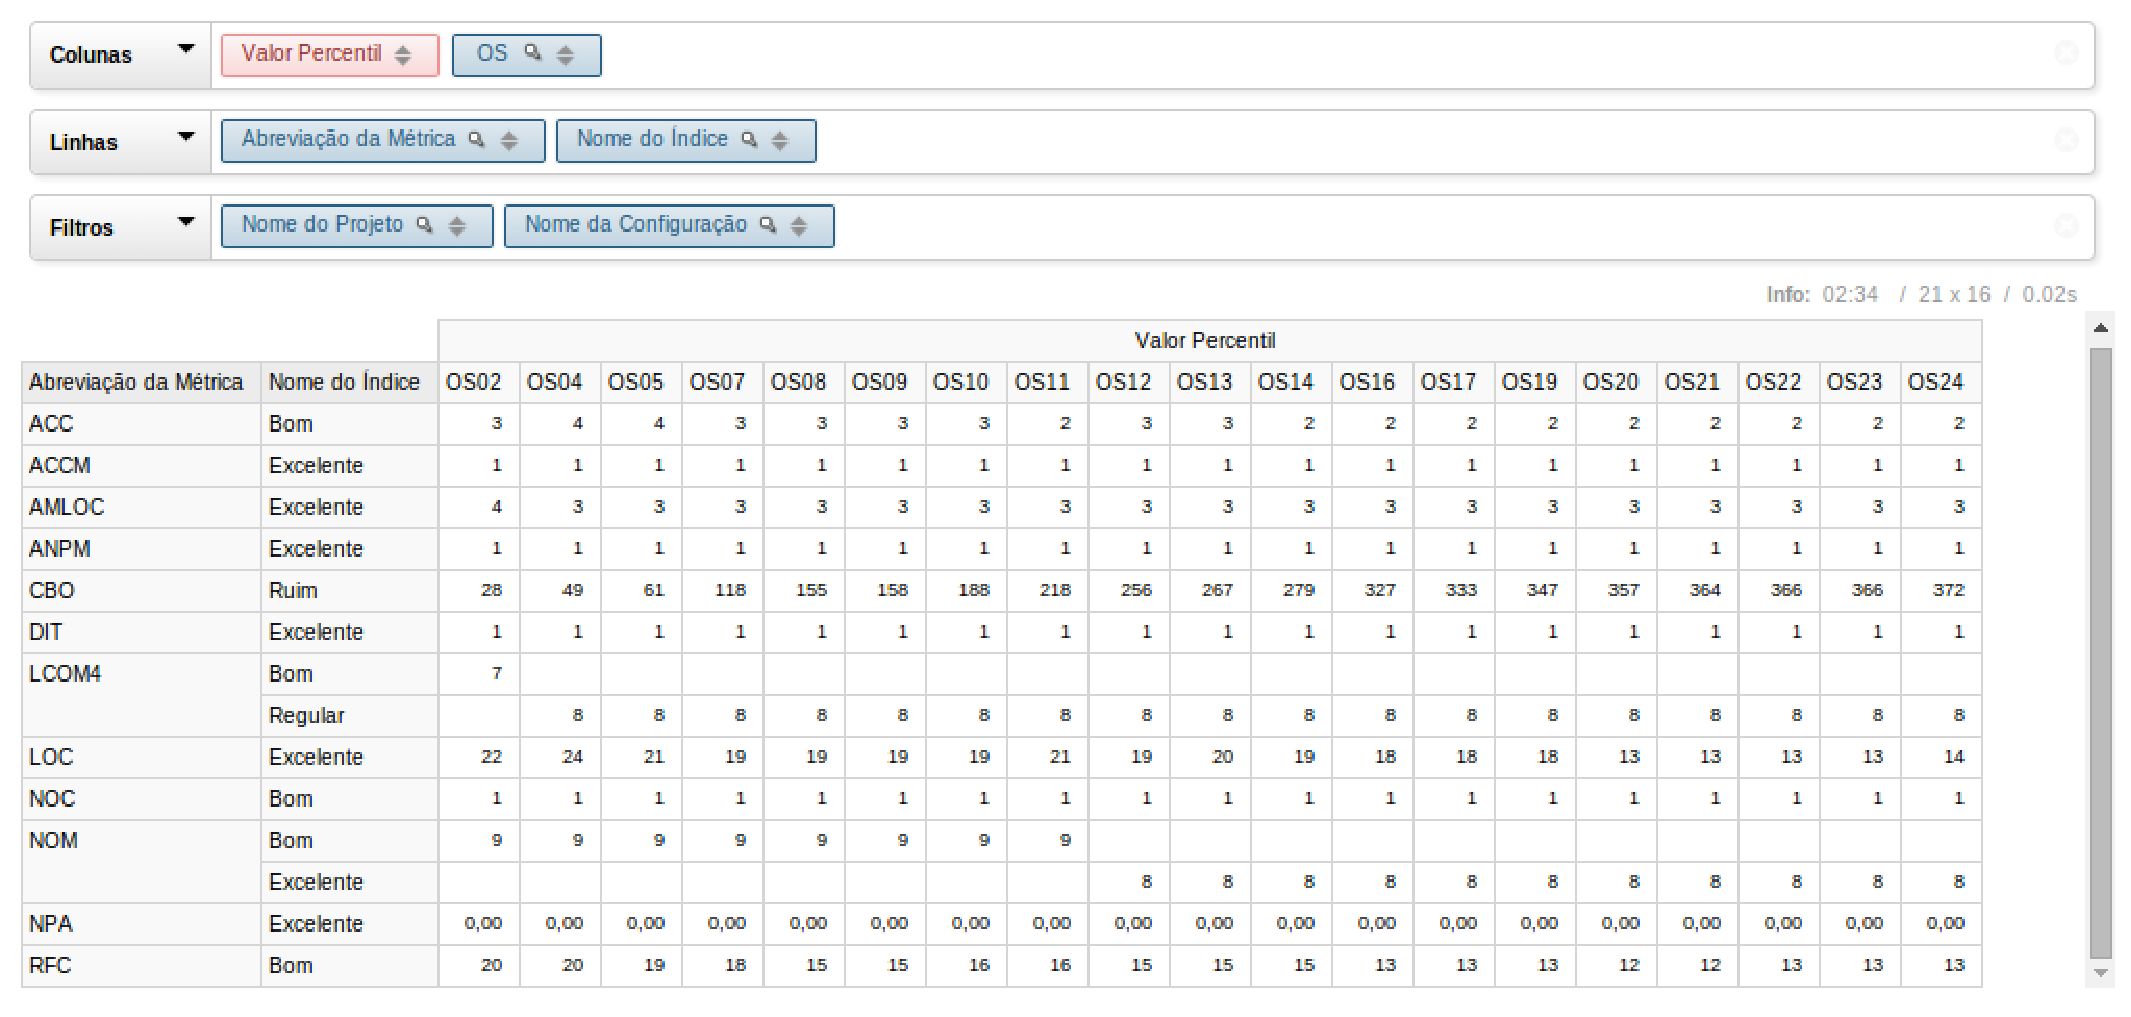
\includegraphics[keepaspectratio=true,scale=0.7]{figuras/total-OpenJDK.eps}
\caption{Interpretação dos valores percentis conforme a configuração "OpenJDK8 Metrics"}
\label{fig:total-openJDK8}
\end{sidewaysfigure}
\FloatBarrier

\begin{sidewaysfigure}[ht!]
\centering
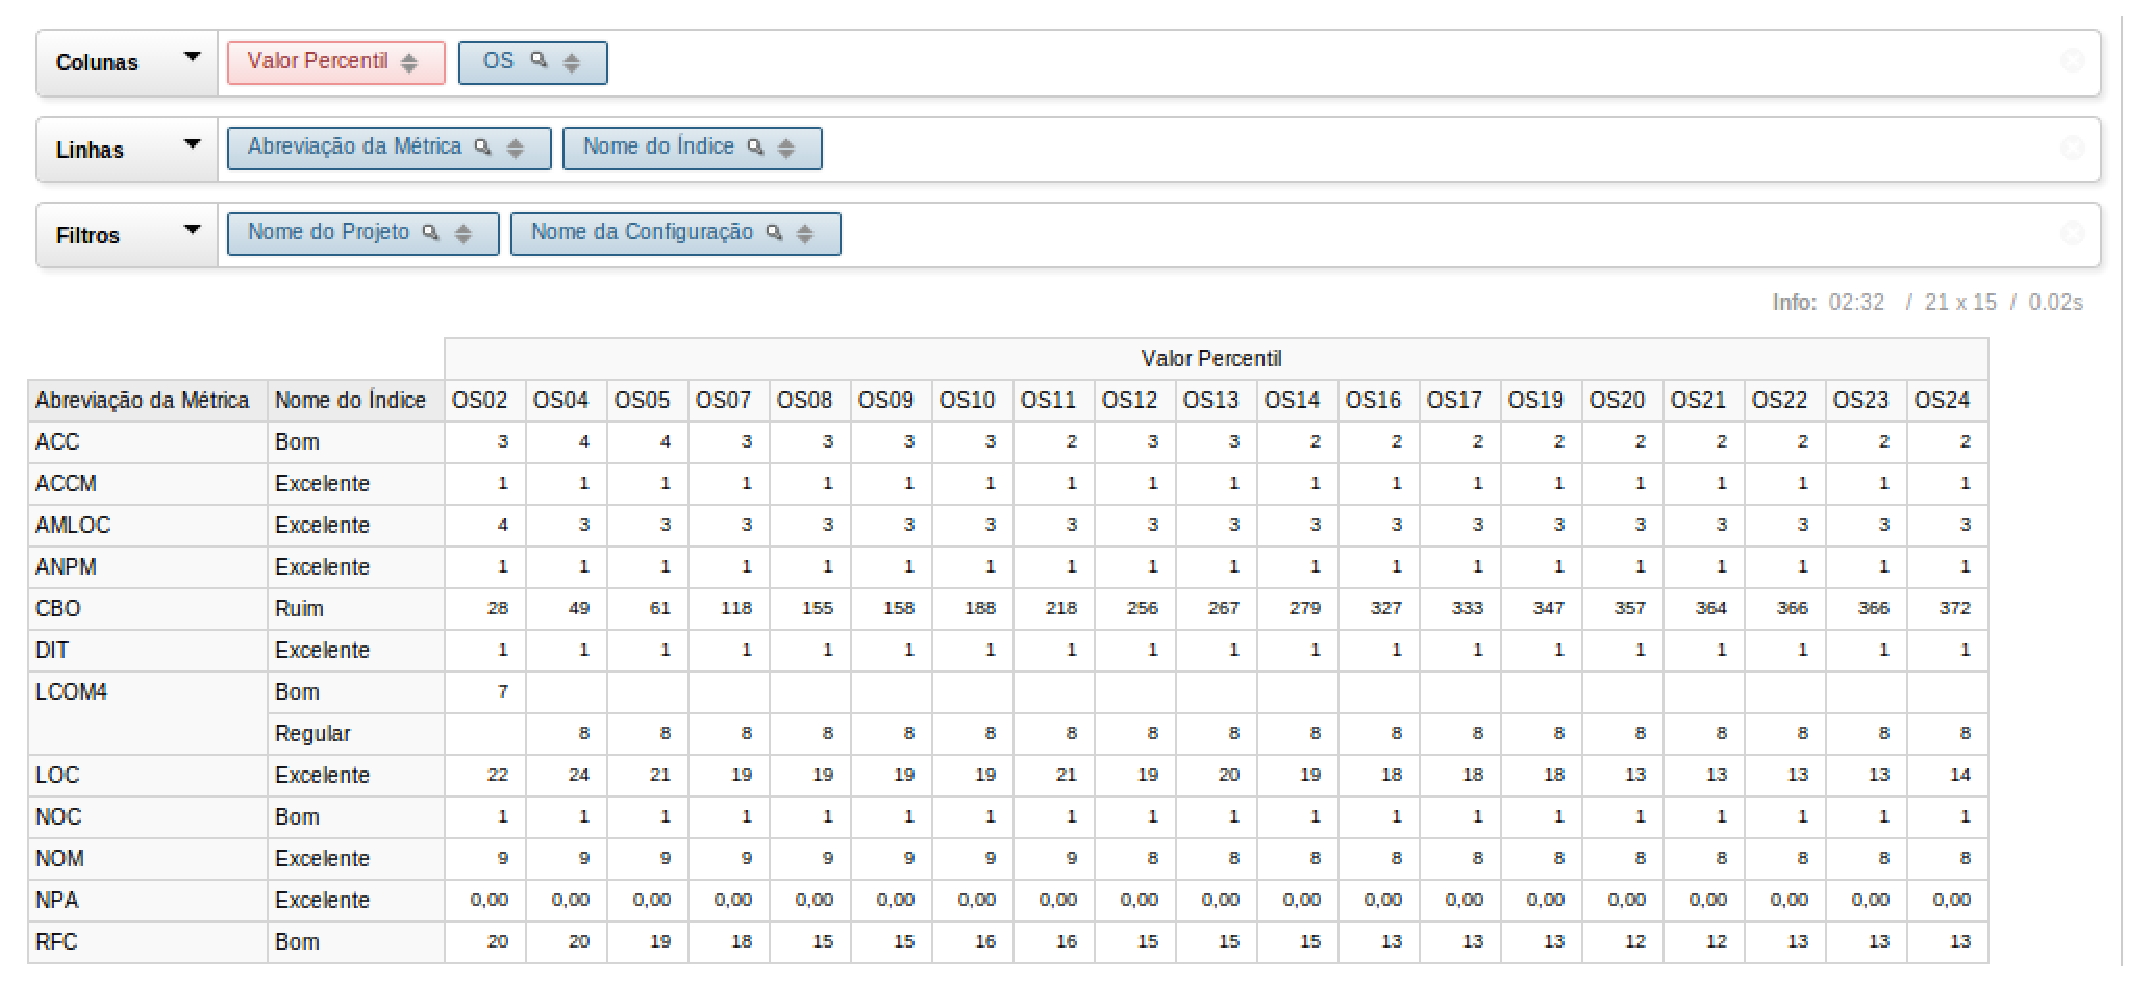
\includegraphics[keepaspectratio=true,scale=0.7]{figuras/total-tomcat.eps}
\caption{Interpretação dos valores percentis conforme a configuração "Tomcat Metrics"}
\label{fig:total-tomcat}
\end{sidewaysfigure}
\FloatBarrier

As métricas \textbf{ACCM, AMLOC, ANPM, DIT, LOC} e \textbf{NPA} permaneceram no intervalo qualitativo~"Excelente"~tanto para a configuração~"OpenJDK8 Metrics"~quanto para a configuração~"Tomcat Metrics", mostrando assim que o software quando comparado com estes softwares de referência, pode-se inferir um bom nível qualidade de código-fonte quanto a estas métricas.

Emboras as métricas \textbf{RFC, ACC e NOC} não alcançaram os valores mais recomendados pelas configurações~"OpenJDK8 Metrics"~e~"Tomcat Metrics", acredita-se que estas estão ainda em patamares considerado aceitáveis segundo as configurações avaliadas. 

Com relação a métrica \textbf{LCOM4}, observa-se que tanto para~"OpenJDK8 Metrics"~quanto para~"Tomcat Metrics", houve uma variação no valor percentil que pode indicar que os métodos estão perdedendo em coesão, justificando assim a mudança da avaliação em~"Bom"~para~"Regular".

Em contraponto a métrica \textbf{LCOM4}, observa-se que a métrica \textbf{NOM} melhorou a avaliação, quando considera-se a configuração~"OpenJDK8 Metrics", de um intervalo qualitativo~"Bom"~para~"Excelente"~podendo assim ser um indício de que as classes estão diminuindo em número de métodos. Em outra avaliação com os resultados obtidos com a métrica \textbf{NOM}, observa-se impacto da avaliação com configurações diferenciadas, onde  os 7 primeiros resultados obtidos com a métrica \textbf{NOM} obtém-se~"Excelente"~para a configuração~"OpenJDK8 Metrics"~e~"Bom"~para~"Tomcat Metrics". Este fato mostra que a configuração escolhida para a avaliação das métricas de código-fonte pode mudar o parâmetro de medição. Dessa forma, recomenda-se escolher sempre um padrão de medição que seja compatível com as funções e natureza da aplicação avaliada.


Observando os valores percentis obtidos para métrica \textbf{CBO}, verifica-se, que para ambas as configurações, o intervalo qualitativo~"Ruim". Embora o valor percentil alto possar ser um indicativo de que o projeto tem um alto fator de acoplamento entre os objetos, verifica-se que o projeto tem um alto grau de utilização de \textit{frameworks} como Hibernate, VRaptor que é um framework construído sobre o framework Spring. Este fato, mostra portanto, que para a métrica \textbf{CBO} é possível considerar o percentil 90 ou avaliar outras configurações que sejam mais adequadas as características do Projeto, pois OpenJDK e Tomcat parecem não ser bom parâmetros de avaliação.  


Visando avaliar também a quantidade de consultas OLAP realizadas no ambiente para atender a esse requisito de negócio, foram contabilizadas 2 consultas OLAP de \textit{Drill Down} sobre as dimensões do Projeto, que são as respectivas Figuras \ref{fig:total-openJDK8} e \ref{fig:total-tomcat}. 

Com intuito de analisar cada uma das métricas, como se mostra nos gráficos e tabelas do Apêndice \ref{graphs}, foram contabilizadas também as operações de análise seletiva: \textit{Slice and Dice} e \textit{Pivoting}. Para cada métrica foram necessários 2 operações\textit{Slice and Dice}; uma para selecionar a configuração e outra para selecionar a métrica desejada e 1 \textit{Pivoting} para se gerar o gráfico em que nas linhas ficavam as \textit{releases} do software.  
 

\subsection{Análise dos Cenários de Limpeza identificados no SICG}

Para analisar os cenários de limpeza de código-fonte, foram extraídas as métricas de código-fonte de cada classe e analisadas conforme a Tabela \ref{tab:cenarios}. Para cada \textit{release}, foram identificados cenários de limpeza de código-fonte conforme a Figura \ref{fig:cenarios-release}.


\begin{figure}[ht!]
\centering
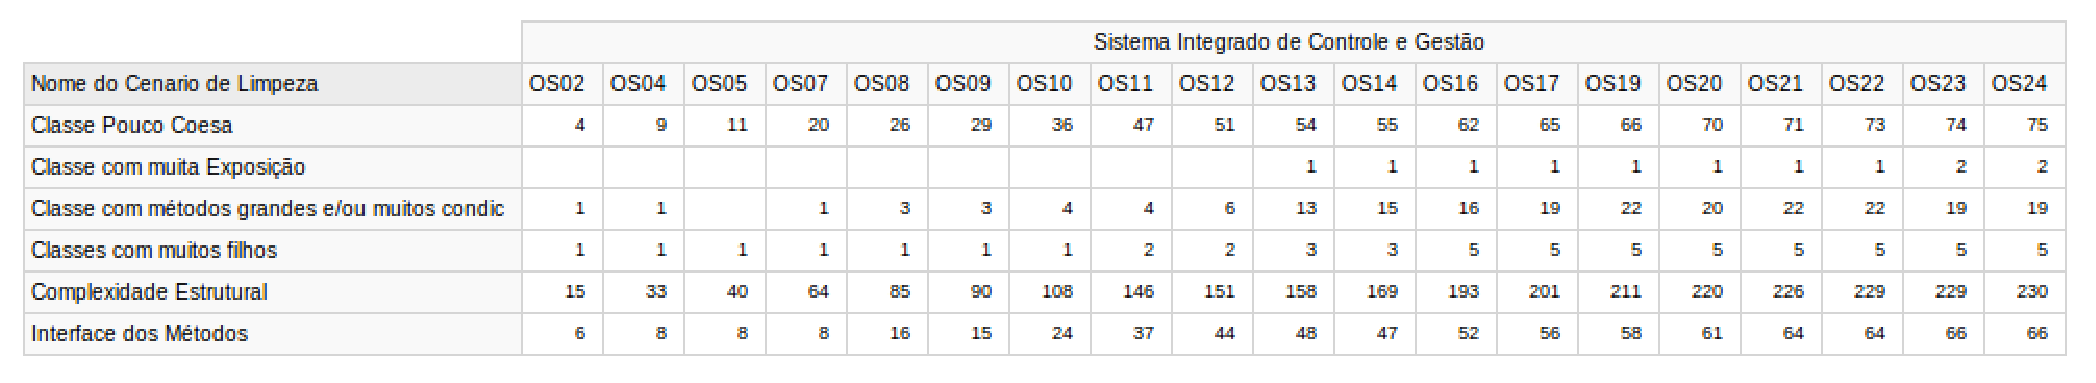
\includegraphics[keepaspectratio=true,scale=0.47]{figuras/total-cenario-tipo.eps}
\caption{Total de Cenários de Limpeza de Código-Fonte identificados por cenário e \textit{Release}}
\label{fig:cenarios-release}
\end{figure}
\FloatBarrier


Realizando uma consuta OLAP de \textit{Drill-Up}, obtém-se uma consolidação do número total de cenários de limpeza por cada uma das releases de software analisadas tal como se observa na Figura \ref{fig:cenarios-total}.

\begin{figure}[ht!]
\centering
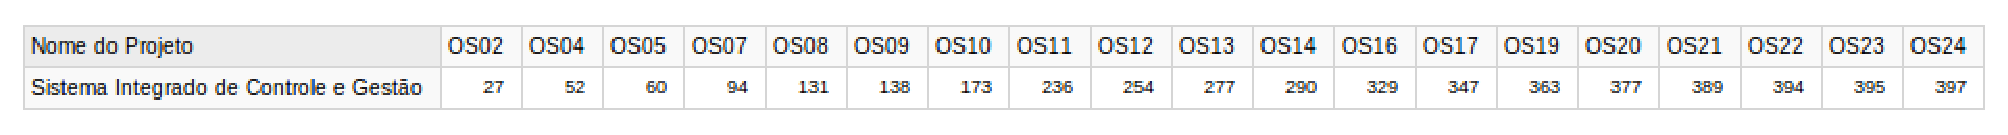
\includegraphics[keepaspectratio=true,scale=0.48]{figuras/total-cenarios-release.eps}
\caption{Total de Cenários de Limpeza de Código-Fonte por Release}
\label{fig:cenarios-total}
\end{figure}
\FloatBarrier

Conforme é possível observar nas Figuras \ref{fig:cenarios-release} e \ref{fig:cenarios-total}, foram detectados mais cenários de limpeza de código-fonte dos tipos \textbf{Complexidade Estrutural}, \textbf{Classe Pouco Coesa} e \textbf{Interface dos Métodos} respectivamente. Os três Cenários de Limpeza com menor número de incidências foram \textbf{Classe com Muita Exposição}, \textbf{Classe com Muitos Filhos} e \textbf{Classe com Métodos Muito Grande e/ou com muitos condicionais}.

No Apêndice \ref{scenarios}, foram detalhadas, para cada um dos cenários de limpeza de código-fonte, para cada uma das \textit{releases}, as classes que contêm os de cenários de limpeza de código de código-fonte. Para realizar esta consulta em cada um dos cenários, foram realizadas uma consulta OLAP de \textit{Drill-Down} e outra de \textit{Slice and Dice}.

Em uma escala de priorização, de qual cenário de limpeza de código-fonte deve ser tratado primeiro, recomenda-se, para o projeto analisado, tratar o cenário de \textbf{Complexidade Estrutural}, pois este sozinho chega a responder entre 55\% a 68\% da quantidade total de cenários identificados. 

Por meio de um \textit{Drill-Down} da consulta OLAP realizada na Figura \ref{fig:cenarios-release} com mais um \textit{Slice and Dice} foram identificadas as 10 classes que apresentaram a maior quantidade de cenários de limpeza e menor quantidade de cenários de limpeza. Os dados podem ser observados nas Figuras \ref{fig:best-10-cenarios} e \ref{fig:worst-10-cenarios} respectivamente.

\begin{figure}[ht!]
\centering
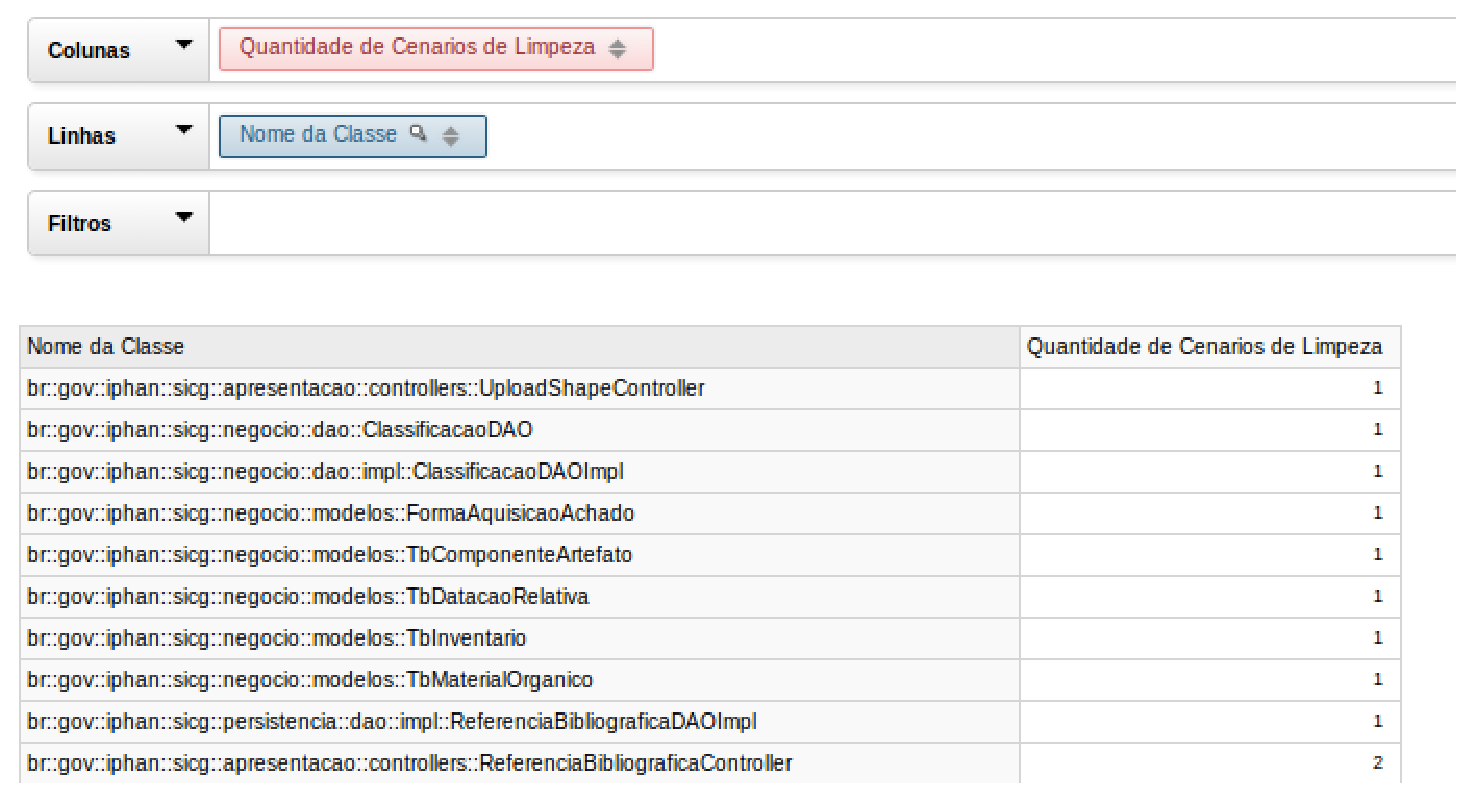
\includegraphics[keepaspectratio=true,scale=0.6]{figuras/10-worst.eps}
\caption{As 10 classes com menor número de Cénarios de Limpeza}
\label{fig:best-10-cenarios}
\end{figure}
\FloatBarrier

\begin{figure}[ht!]
\centering
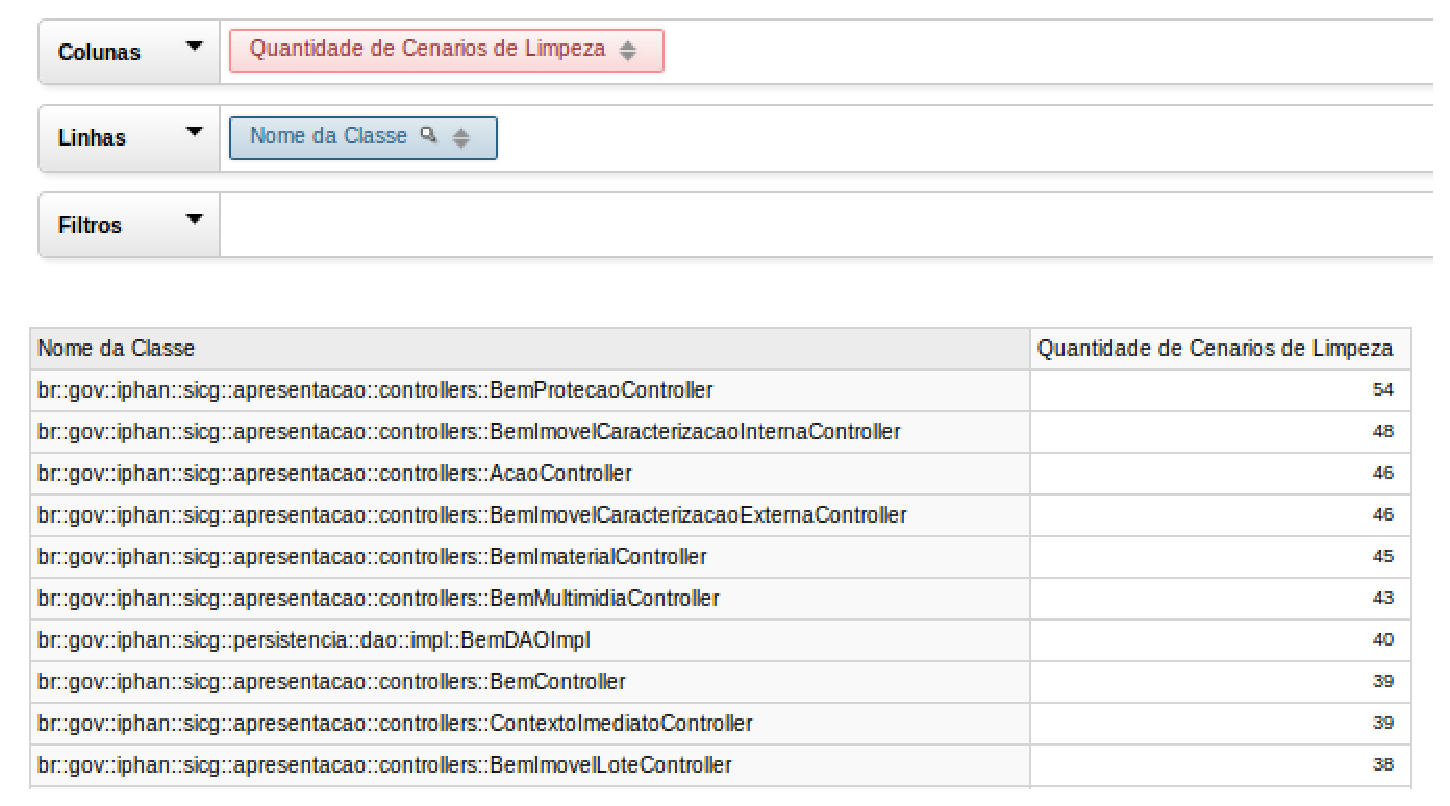
\includegraphics[keepaspectratio=true,scale=0.6]{figuras/10-best.eps}
\caption{As 10 classes com maior número de Cénarios de Limpeza}
\label{fig:worst-10-cenarios}
\end{figure}
\FloatBarrier


\subsection{Análise da Taxa de Aproveitamento de Oportunidade de Melhoria de Código-Fonte}

A partir da identificação dos cenários de limpeza de código-fonte e da contagem do número de classes em uma determinada \textit{release} do software, foi possível calcular a Taxa de Aproveitamento de Oportunidade de Melhoria de Código-Fonte conforme a fórmula \ref{eqn01}.

\begin{equation}
\label{eqn01}
T_r =   \frac{{\sum_{i=1}^{n}{Ce_i}}}{\sum_{i=1}^{n}{Cl_i}}
\end{equation}

onde $ Ce $ é o total de cenário de limpeza e $ Cl $ é a quantidade classes.

 Embora se pudesse realizar o cálculo acima, utilizando a consulta que realiza o \textit{Drill-Up} nas dimensões, Figura \ref{fig:cenarios-total}, preferimos consolidar o fato do número de cenários de limpeza de uma determinada release, em uma outra tabela fato. Como explicado na Seção \ref{sec:project-dw}, \citeonline{Kimball2002} recomenda que medidas de proporção, como taxas, que são fatos não aditivos, devam estar na mesma tabela que o numerador e denominador.

 Dessa forma, ao se realizar uma consulta OLAP de \textit{Drill Down} nas dimensões associadas, obteve-se a Taxa de Aproveitamento de Oportunidade de Melhoria de Código-Fonte por cada release do software conforme se mostra nas Figuras \ref{fig:taxa-cenarios} e \ref{fig:grafico-taxa} e o crescimento do projeto conforma a Figura \ref{fig:crescimento-projeto}. 


\begin{figure}[H]
\centering
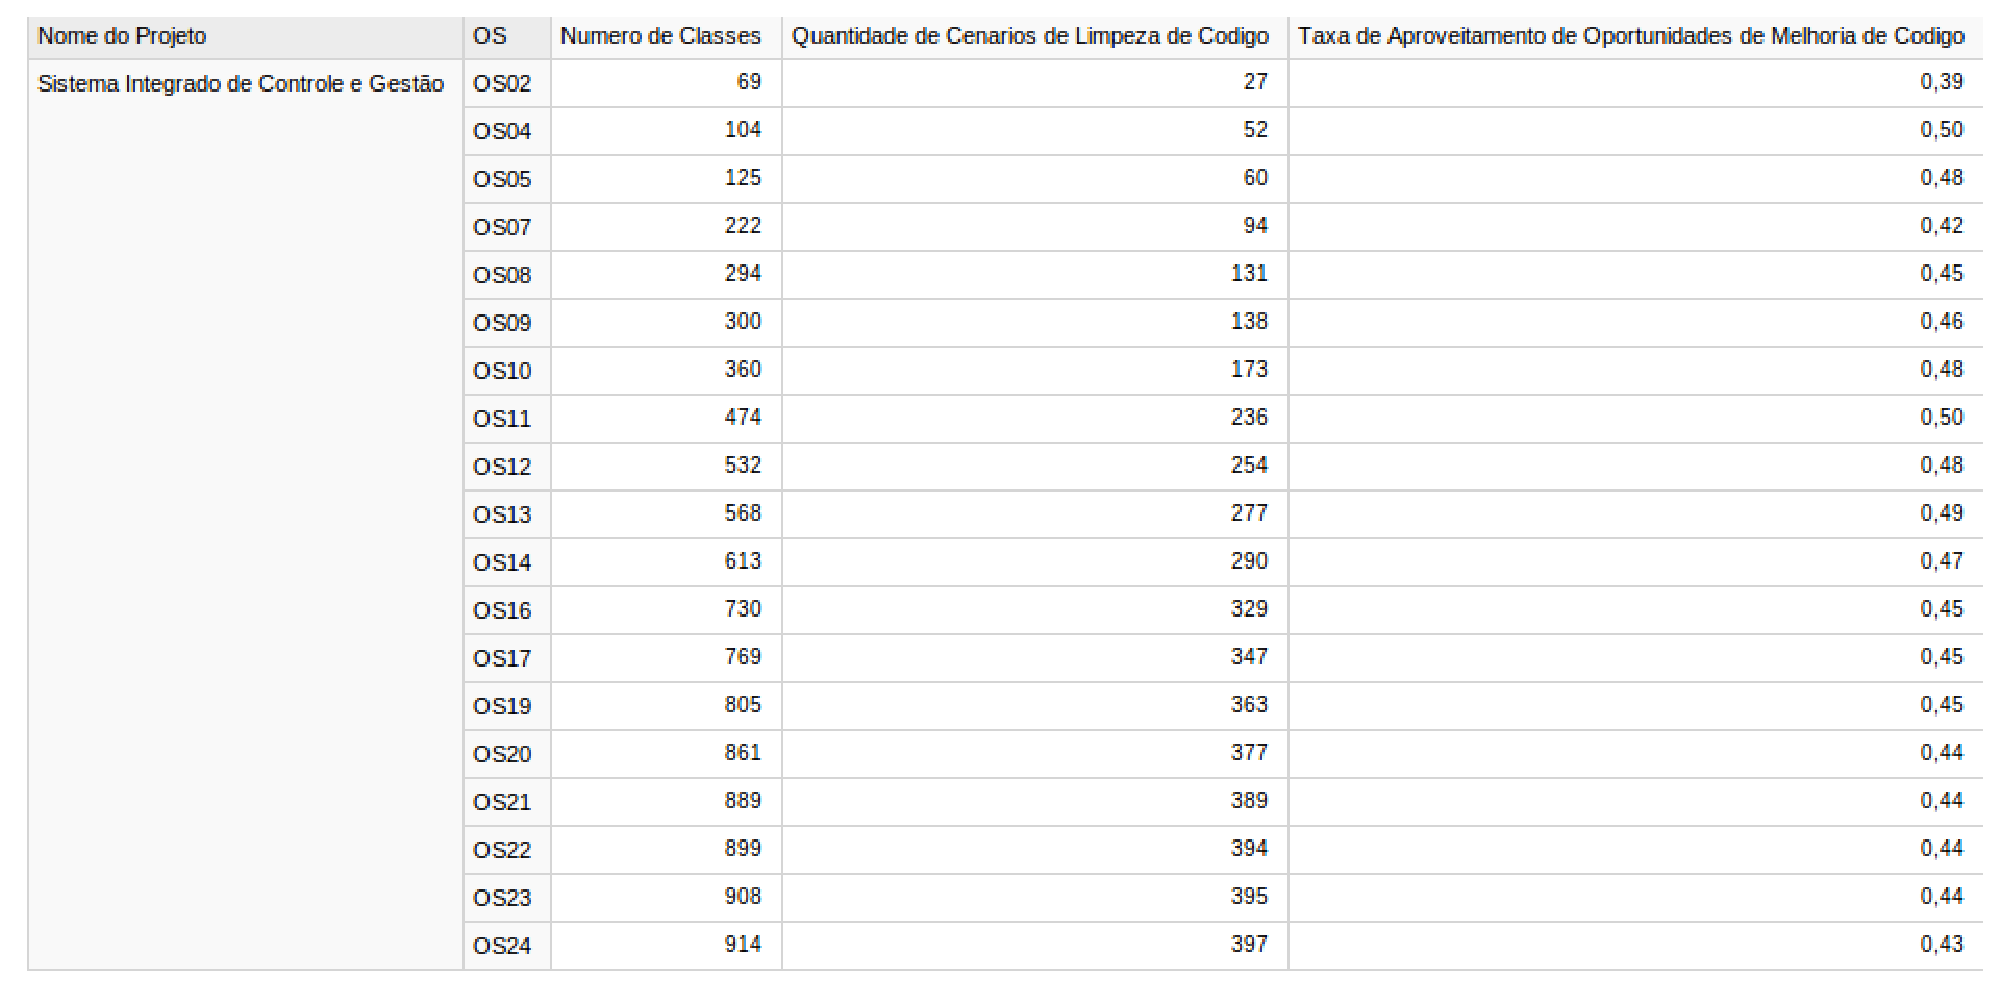
\includegraphics[keepaspectratio=true,scale=0.48]{figuras/taxa-parcial.eps}
\caption{Taxa de Aproveitamento de Oportunidades de Melhoria de Código-Fonte}
\label{fig:taxa-cenarios}
\end{figure}
\FloatBarrier


\begin{figure}[H]
\centering
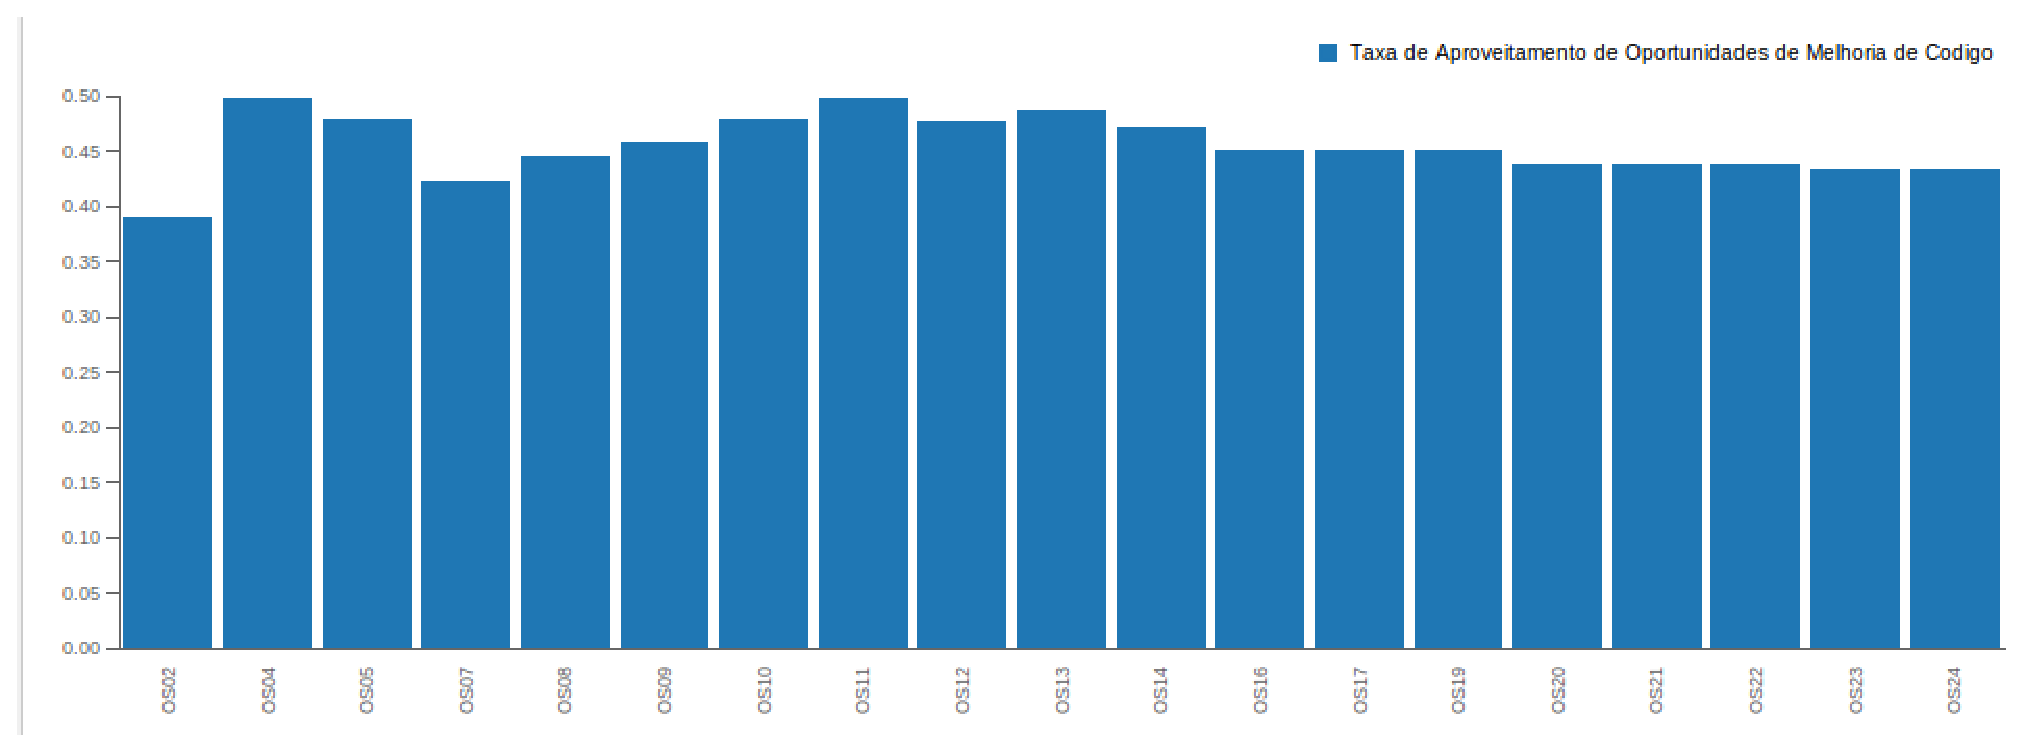
\includegraphics[keepaspectratio=false,scale=0.48]{figuras/taxa-grafico.eps}
\caption{Gráfico da Taxa de Aproveitamento de Oportunidades de Melhoria de Código-Fonte}
\label{fig:grafico-taxa}
\end{figure}
\FloatBarrier

\begin{figure}[H]
\centering
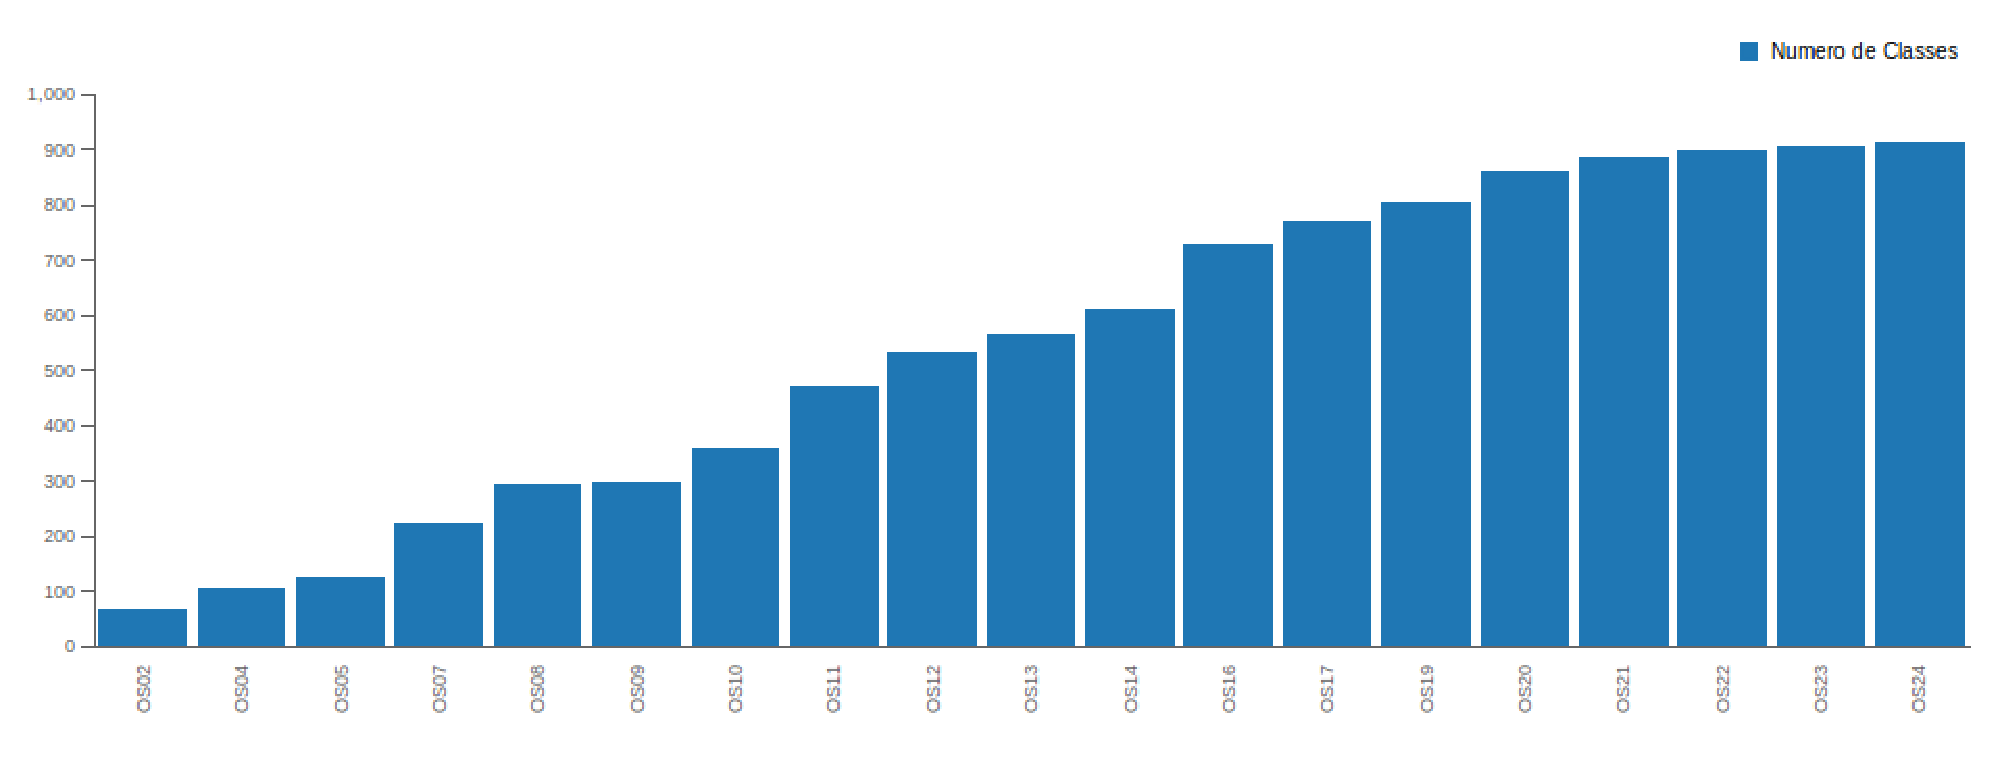
\includegraphics[keepaspectratio=false,scale=0.48]{figuras/crescimento-projeto.eps}
\caption{Crescimento do número de Classes do Projeto SICG}
\label{fig:crescimento-projeto}
\end{figure}
\FloatBarrier


Utilizando as Figuras \ref{fig:taxa-cenarios} e \ref{fig:grafico-taxa}, observa-se que o projeto cresceu de 67 classes, na primeira release, para 914 classes ao final da última release e o número total de cenários de limpeza de código-fonte identificados cresceu de 27 para 397. Ao se realizar cálculo da Taxa de Aproveitamento de Oportunidade de Melhoria de Código-Fonte, observou-se que há uma tendência de que esta taxa se mantenha entre 0,4 a 0,5. Este fato pode indicar duas hipóteses: a primeira de que o projeto cresceu em uma taxa muito maior que a quantidade de cenários de limpeza, indicando assim uma estabilidade na complexidade do projeto; ou que não foram promovidas atividades de melhoria de código-fonte ao longo das 24 releases.  

